
\documentclass{beamer}
\usepackage[utf8]{inputenc}
\usetheme{focus} % Use the Focus theme supplied with the template
% Add option [numbering=none] to disable the footer progress bar
% Add option [numbering=fullbar] to show the footer progress bar as always full with a slide count

% Uncomment to enable the ice-blue theme
%\definecolor{main}{RGB}{92, 138, 168}
%\definecolor{background}{RGB}{240, 247, 255}

%------------------------------------------------

\usepackage{booktabs} % Required for better table rules

%----------------------------------------------------------------------------------------
%	 TITLE SLIDE
%----------------------------------------------------------------------------------------

\title{Word Count Problem \& \\Cross Correlation Calculation}

\subtitle{Solutions Diagram and Entity Interaction}

\author{Filipe Pires | 85122 | filipesnetopires@ua.pt \\ João Alegria | 85048 | joao.p@ua.pt}

\institute{University of Aveiro, DETI}

\date{\today}

%------------------------------------------------

\begin{document}

%------------------------------------------------

\begin{frame}
	\maketitle % Automatically created using the information in the commands above
\end{frame}

%----------------------------------------------------------------------------------------
%	 WORD COUNT
%----------------------------------------------------------------------------------------

\section{Word Count Problem}

%------------------------------------------------

\begin{frame}{Multi-Thread Mapping}
	The team efforts were focused on mapping the initial single-threaded implementation of the program to a multi-threaded environment.
	The required mapping was:
	\begin{itemize}
		\item A shared memory space would keep track of the files to be processed.
		\item Each worker thread would ask the shared memory for a chunk of text, process it and return the results to the shared memory.
		\item The shared memory would manage the files' content internally, enabling the distribution of chunks of text.
		\item The shared memory would keep track of all received results, enabling a print in the end of the global results processing of each file given as input.
	\end{itemize}
\end{frame}

%------------------------------------------------

\begin{frame}{Solution Diagram}
	\begin{figure}
		\includegraphics[width=6cm]{wordCountDiagram.png}
		\caption{Solution Diagram}
		\label{wordDiagram}
	\end{figure}
\end{frame}

%------------------------------------------------

\begin{frame}{Entity Interaction}
	\begin{figure}
		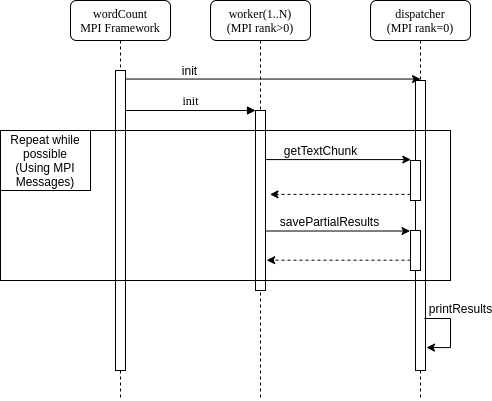
\includegraphics[width=6cm]{wordCountInteraction.png}
		\caption{Entity Interactions}
		\label{wordInteraction}
	\end{figure}
\end{frame}

%----------------------------------------------------------------------------------------
%	 CROSS CORRELATION CALCULATION
%----------------------------------------------------------------------------------------

\section{Cross Correlation Problem}

%------------------------------------------------

\begin{frame}{Multi-Thread Mapping}
	Once again, our task was to map a single-threaded implementation of the solution for this second problem, previously developed by us, to a multi-threaded
	version of such implementation.
	The required mapping was:
	\begin{itemize}
		\item A shared memory space would keep track of the files to be processed.
		\item Each worker thread would ask the shared memory for the values of a signal and a specific $\tau$, calculate the cross correlation and return the results to the shared memory.
		\item The shared memory would manage the files' content internally, enabling the distribution of the same signals but with different $\tau$ values.
		\item The shared memory would keep track of all received results, enabling the program to write the results in the end of each file or to print them to the console.
	\end{itemize}
\end{frame}

%------------------------------------------------

\begin{frame}{Solution Diagram}
	\begin{figure}
		\includegraphics[width=5cm]{crossCorrelationDiagram.png}
		\caption{Solution Diagram}
		\label{crossDiagram}
	\end{figure}
\end{frame}

%------------------------------------------------

\begin{frame}{Entity Interaction}
	\begin{figure}
		\includegraphics[width=6cm]{crossCorrelationInteraction.png}
		\caption{Entity Interactions}
		\label{crossInteraction}
	\end{figure}
\end{frame}

\end{document}
